% Sidebar subcategory icon: Fields — contour bands across a domain, the generic
% picture of a field defined over a mesh. Distinct from `fieldCalc` (a table of
% values), `average` (a transfer arrow) and `levelset` (a single thick interface
% splitting a shaded domain).
% Two bands, not three: at the 14px a .sb-subsection-header renders this at, a
% third band leaves under a pixel of gap and the three merge into a grey block.
% NOTE: the committed svg-ui/catFields.svg was hand-authored to the same drawing
% (no pdftocairo available); regenerating via `make ui` replaces it with the
% pdftocairo rendering of this source — same glyph either way.
\documentclass[tikz,border=2mm]{standalone}
\usetikzlibrary{arrows.meta,calc,shapes.geometric}
\begin{document}
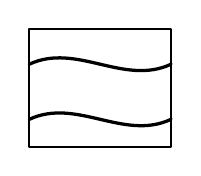
\begin{tikzpicture}[line width=1.3pt, line cap=round, line join=round, x=1mm,y=1mm]
  \draw[thick] (-9,-7.5) rectangle (9,7.5);
  \draw[line width=1.18pt] (-9,3) .. controls (-3,5.8) and (3,0.2) .. (9,3);
  \draw[line width=1.18pt] (-9,-4) .. controls (-3,-1.2) and (3,-6.8) .. (9,-4);
\end{tikzpicture}
\end{document}
